\chapter{Projects}

\section{STM32 IMU}
\subsection{PModNav}
The purpose is to get the \texttt{roll}, \texttt{pitch} and \texttt{yaw} from the PModNav to plot a 3D visualization of the IMU. The final purpose of it is to create log files from the orientation and attitude of the drone in real-time. By combining data from accelerometers, gyroscopes and magnetometers, an IMU can provide information about the object's position, orientation and angular velocity. This is crucial for tasks such as safety deployement or drone tracking.
The STM32-L4796ZG recovers the value of the sensors from the \texttt{PModNav} via \texttt{SPI Bus} and transmits them to the HMI via \texttt{UART} connection.
\begin{figure}[H]
    \centering
    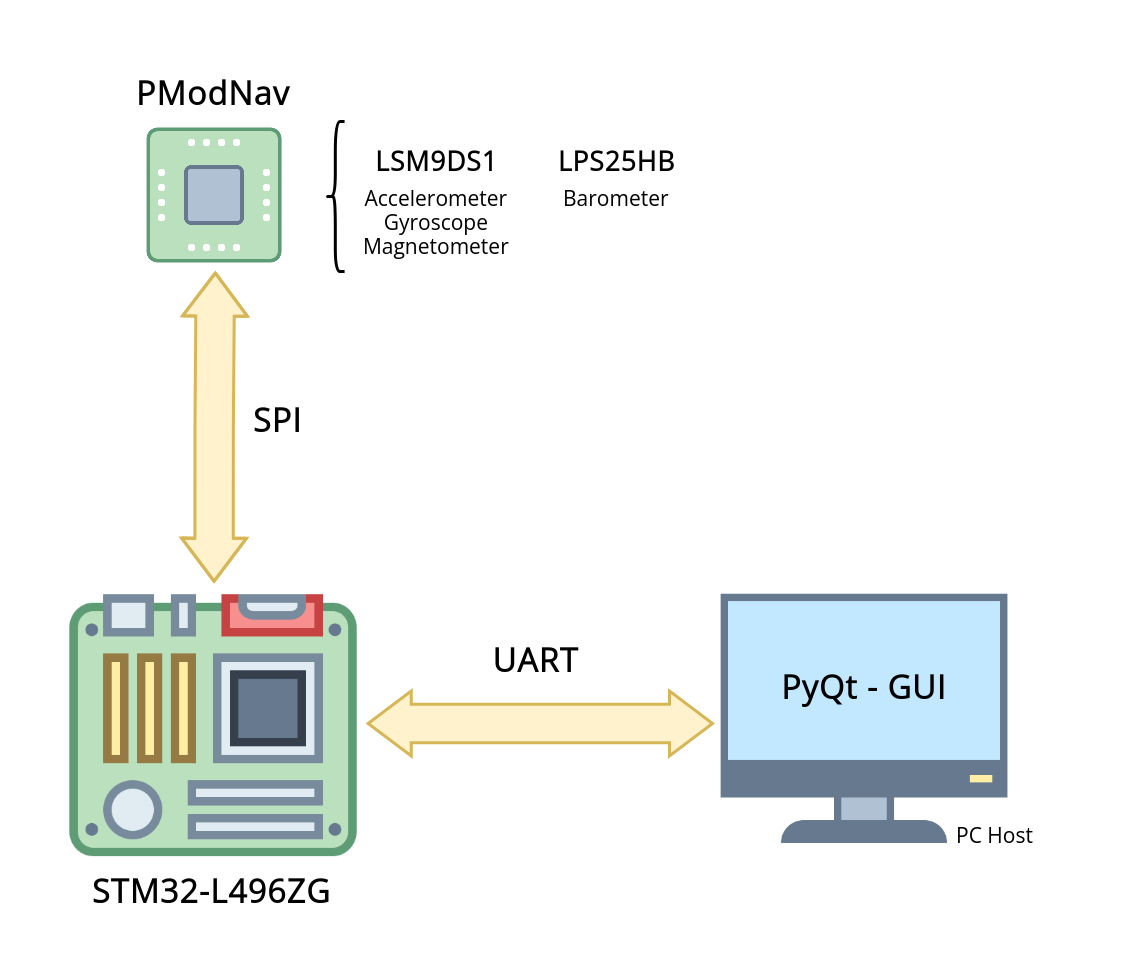
\includegraphics[width=0.65\linewidth]{./projects/pmodnav/com.png}
    \caption{Project communication overview}
\end{figure}

\subsubsection{Hardware}
The PModNav module is equipped with the \texttt{LSM9DS1}\cite{LSM9DS1_digilent_lib} sensor, offering 10-degrees-of-freedom (10-DOF) functionality. It integrates a 3-axis accelerometer, 3-axis gyroscope, 3-axis magnetometer, and an LPS25HB digital barometer. This comprehensive sensor suite allows users to obtain orientation-related data and determine the precise position and heading of the module. The module supports various full-scale options for linear acceleration, angular rate, and magnetic field measurements. It follows the Digilent Interface Specification Type 2A and utilizes a 12-pin Pmod connector with an SPI interface.

\subsubsection{Software and Development Environment}
The development environment for the PModNav project is STM32 CubeIDE. The documentation references project sources, including code snippets and libraries, such as the PModNav driver and Madgwick's filter implementation. 

\subsubsection{Data Processing}
The project outlines two approaches for deriving object attitudes: Euler angles and quaternions. Euler angles are obtained through the integration of angular velocity and provide information about the roll, pitch, and yaw of an object. However, a challenge known as \texttt{Gimbal Lock}\cite{gimbal_lock} arises when using Euler angles directly, resulting in a loss of a degree of freedom when two axes of rotation overlap. To overcome this, quaternions are introduced as a mathematical representation of displacement and rotation. They effectively resolve the Gimbal Lock issue and provide a more robust solution for determining attitudes.
\begin{figure}[H]
    \centering
    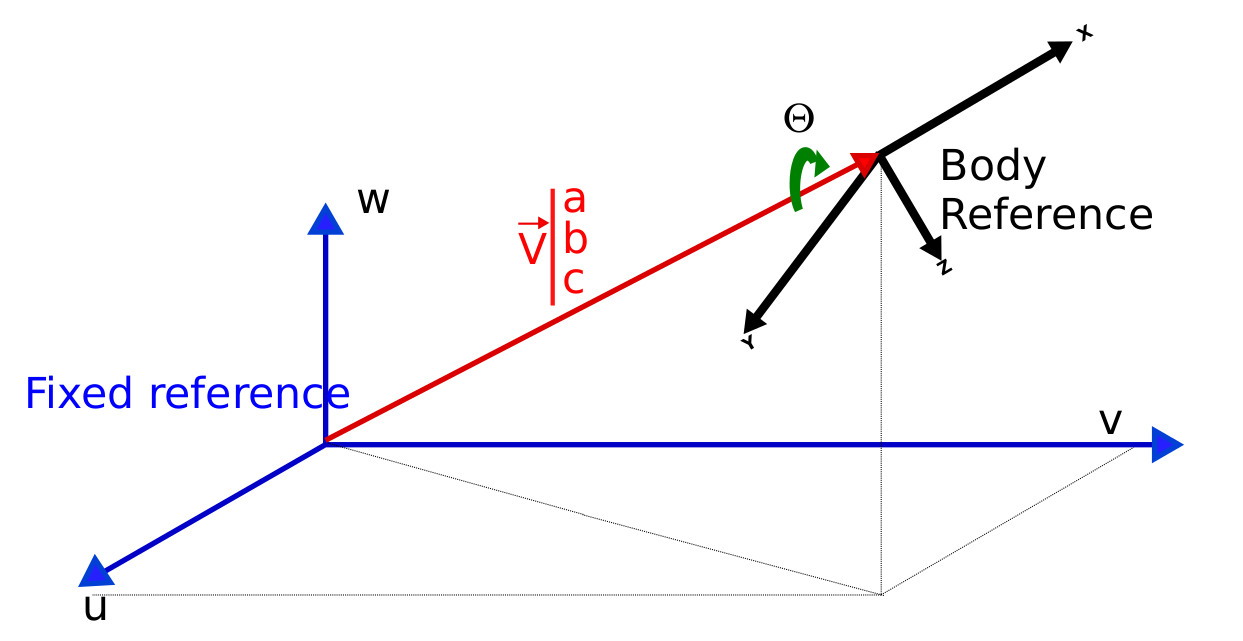
\includegraphics[width=0.65\linewidth]{./projects/pmodnav/quaternions.png}
    \caption{Quaternion representation}
\end{figure}
$$ Q = [q_0, q_1, q_2, q_3 ] $$
$$ Q = \big[cos(\frac{\theta}{2}), a.sin(\frac{\theta}{2}), b.sin(\frac{\theta}{2}), c.sin(\frac{\theta}{2})\big] $$
At each \texttt{Te}, we can calculate the new value of the quaternion vector from the velocity :
$$ Q_{k+1} = Q_k+\frac{1}{2}.T_e.\omega_k.Q_k $$
For cheap IMUs, it is unavoidable to perform a data fusion to make the accelerometer compensate for the gyroscope defect. If using a Kalmann filter is possible, there are other (faster) algorithms like Madgwick's. The idea is to compensate for the gyroscope measurement error by modulating its values by the result of a comparison between an estimate of the gravity field and the measured gravity field (with the accelerometer).
\begin{figure}[H]
    \centering
    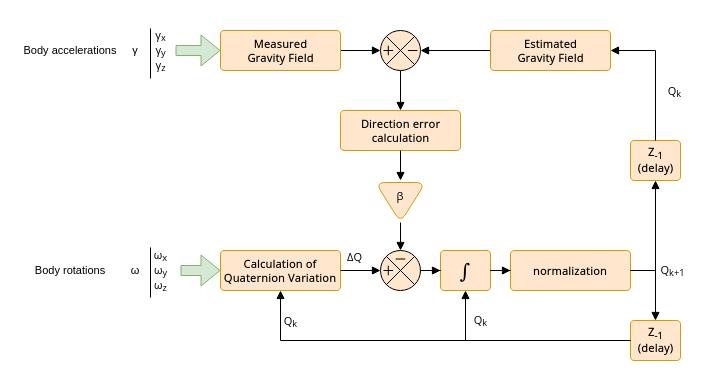
\includegraphics[width=0.9\linewidth]{./projects/pmodnav/madgwick.png}
    \caption{Madgwick filter schematic}
\end{figure}
I decided to use the most popular open source algorithm to compute rotations, the \texttt{Madgwick's algorithm}\cite{Madgwick}. This calculation updates the quaternion, from which the attitudes (Euler angles) can be calculated.
\begin{figure}[H]
    \centering
    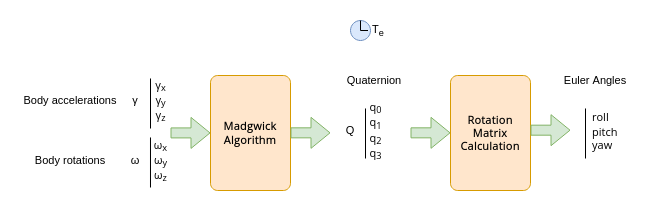
\includegraphics[width=0.9\linewidth]{./projects/pmodnav/madgwick_applied.png}
    \caption{Data transform schematic}
\end{figure}
$$ R_{12} = 2.(q_1.q_2+q_0.q_3) $$
$$ R_{22} = q_0^2+q_1^2-q_2^2-q_3^2 $$
$$ R_{31} = 2.(q_0.q_1+q_2.q_3) $$
$$ R_{32} = 2.(q_1.q_3-q_0.q_2) $$
$$ R_{33} = q_0^2-q_1^2-q_2^2+q_3^2 $$
Calculation of the Euler Angles from the rotation matrix :
$$ roll = atan2(R_{31},R_{33}) $$
$$ pitch = asin(R_{32}) $$
$$ yaw = atan2(R_{12},R_{22}) $$


\subsection{Graphical User Interface}
Additionally, a graphical user interface (GUI) is provided, leveraging \texttt{PyQt5}\cite{pyqt5} and \texttt{PyOpenGL}\cite{pyopengl} modules. The GUI manages the main window and handles OpenGL object management. It offers features like port selection and serial communication. The received data is displayed in a textbox within the GUI, facilitating real-time monitoring and analysis.
Here is how the GUI is threaded :
\begin{figure}[H]
    \centering
    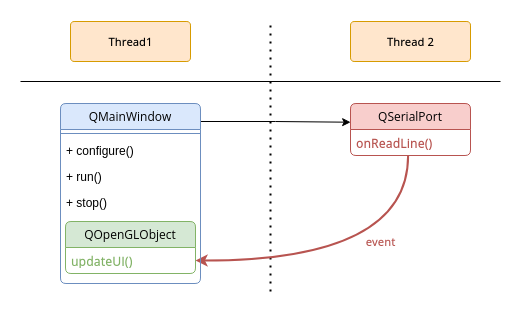
\includegraphics[width=0.65\linewidth]{./projects/pmodnav/gui_threads.png}
    \caption{Python GUI threads schematic}
\end{figure}
The use is rather simple for the communication configuration (\colorbox{cyan}{cyan box}) :
\begin{itemize}
    \item the port
    \item the baud rate
    \item the number of bits per frame
    \item the number of stop bits
    \item the parity
    \item the flow control
\end{itemize}
\begin{figure}[H]
    \centering
    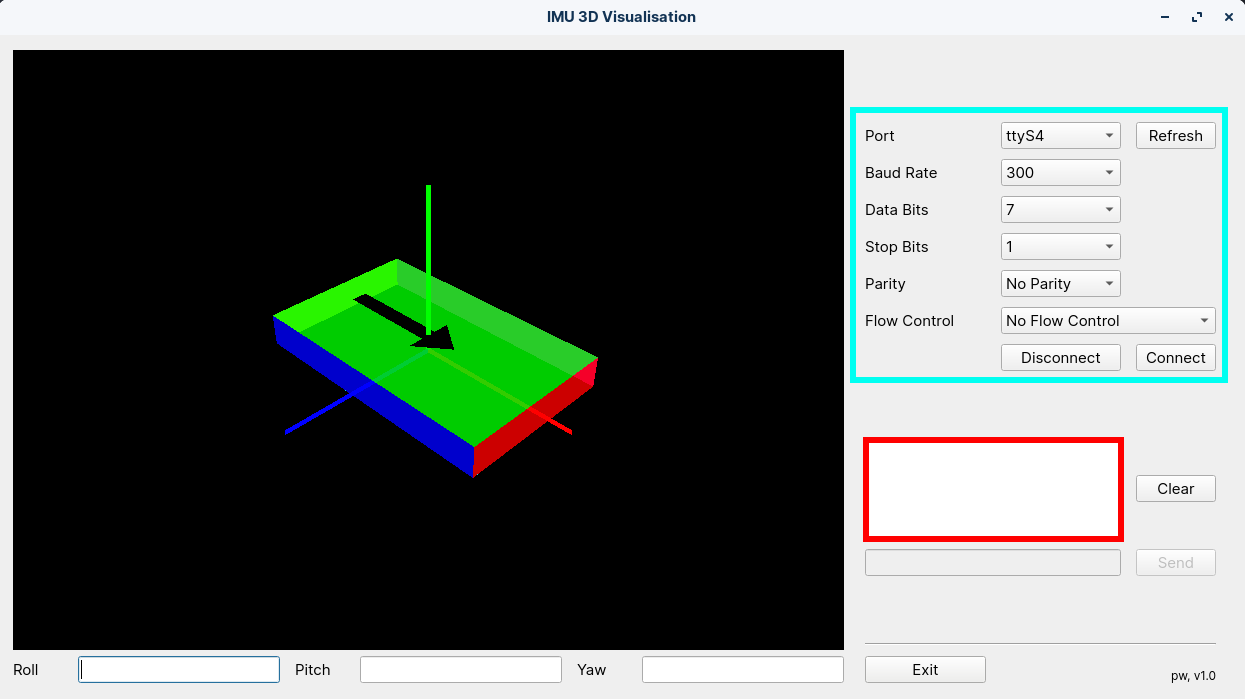
\includegraphics[width=0.65\linewidth]{./projects/pmodnav/gui_window.png}
    \caption{Python GUI window screenshot}
\end{figure}
Then click on \texttt{Connect} to start the serial communication. Every received line appeared in the textBox (\colorbox{red}{red box}).

\subsubsection{Final result}
% \begin{figure}[H]
%     \centering
%     \includegraphics{./projects/pmodnav/pmodnav_gui_record.gif}
%     \caption{Python GUI window GIF}
% \end{figure}

\subsection{Telemetry data}


\section{LogViewer}
The objective of a log viewer application is to facilitate the efficient viewing and analysis of log data generated by systems or applications. This scientific report highlights the key goals and functionality of a log viewer, which includes log visualization, search and filtering capabilities, log analysis and insights, integration with other tools, and customization options.
\subsection{Sensors tests}

\begin{figure}[H]
    \centering
    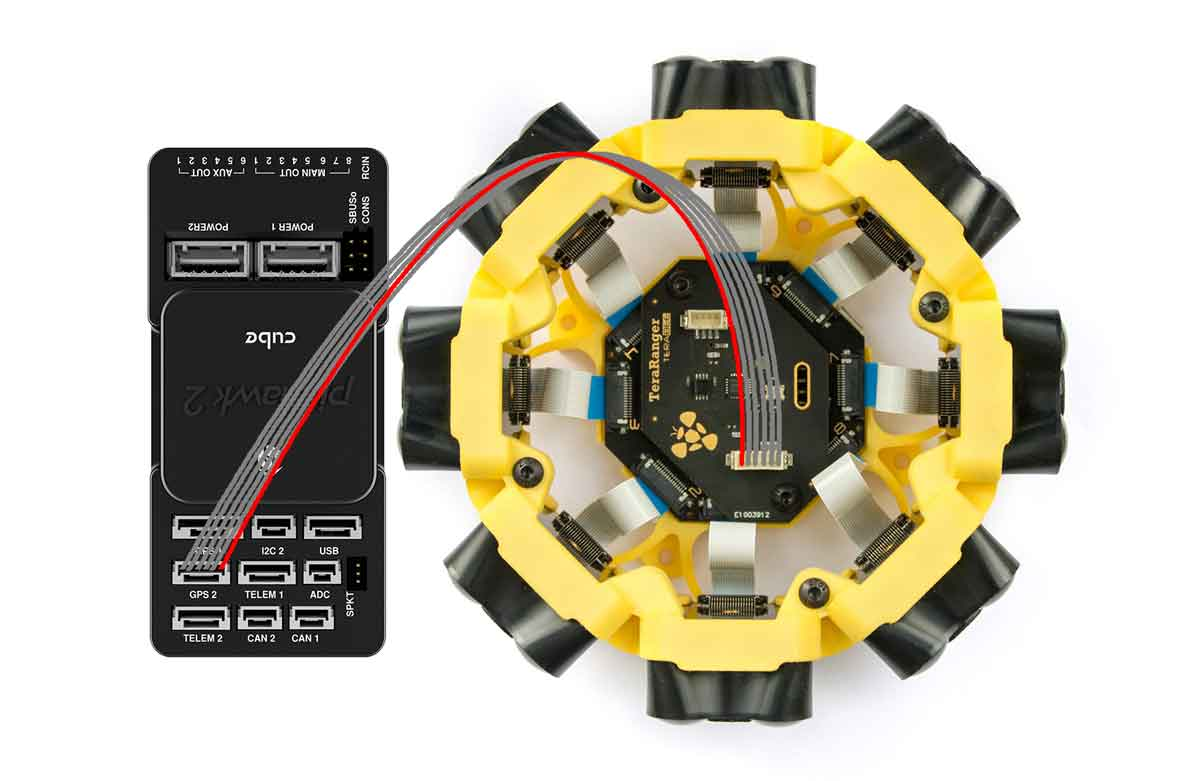
\includegraphics[width=0.65\linewidth]{./projects/logviewer/tower_evo_pixhawk.jpg}
    \caption{Terabee TowerEvo sensors and Pixhawk FlightController}
\end{figure}


\begin{table}[H]
    \centering
    \begin{tabular}{|l||l|l|}
    \hline
                      & TowerEvo & Description                 \\
    \hline
    PRX\_ORIENT       & 0        & Default                     \\
    PRX\_TYPE         & 6        & TeraRangerTowerEvo          \\
    SERIAL\_BAUD      & 921600   & serial baud                 \\
    SERIAL\_PROTOCOLE & 11       & Lidar 360 deg               \\
    AVOID\_ANGLE      & 1300     & max  lean angle             \\
    AVOID\_BEHAVE     & 1        & Stop when obstacle detected \\
    AVOID\_DIST\_MAX  & 5        & max distance avoidance      \\
    AVOID\_ENABLE     & 3        & Enable drone reaction       \\
    AVOID\_MARGIN     & 3        & min distance avoidance      \\
    \hline
    \end{tabular}
    \caption{Ardupilot flight controller configuration}
    \label{table:fc_config}
\end{table}

\begin{figure}[H]
    \centering
    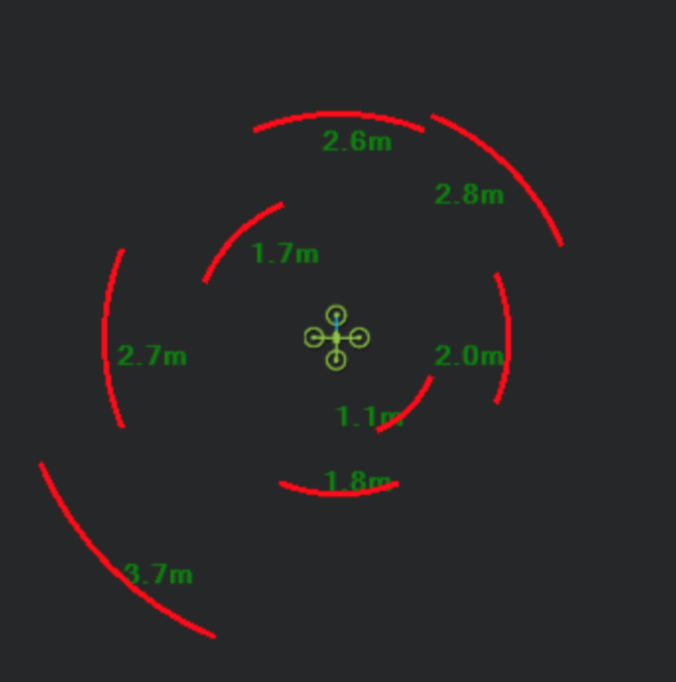
\includegraphics[width=0.3\linewidth]{./projects/logviewer/mission_planner_tower_evo.png}
    \caption{Data acquisition acknowledgement}
\end{figure}

\subsection{Sensors Integration and drone flight}
Drone integration
\begin{figure}[H]
    \centering
    \begin{subfigure}[b]{0.475\textwidth}
        \centering
        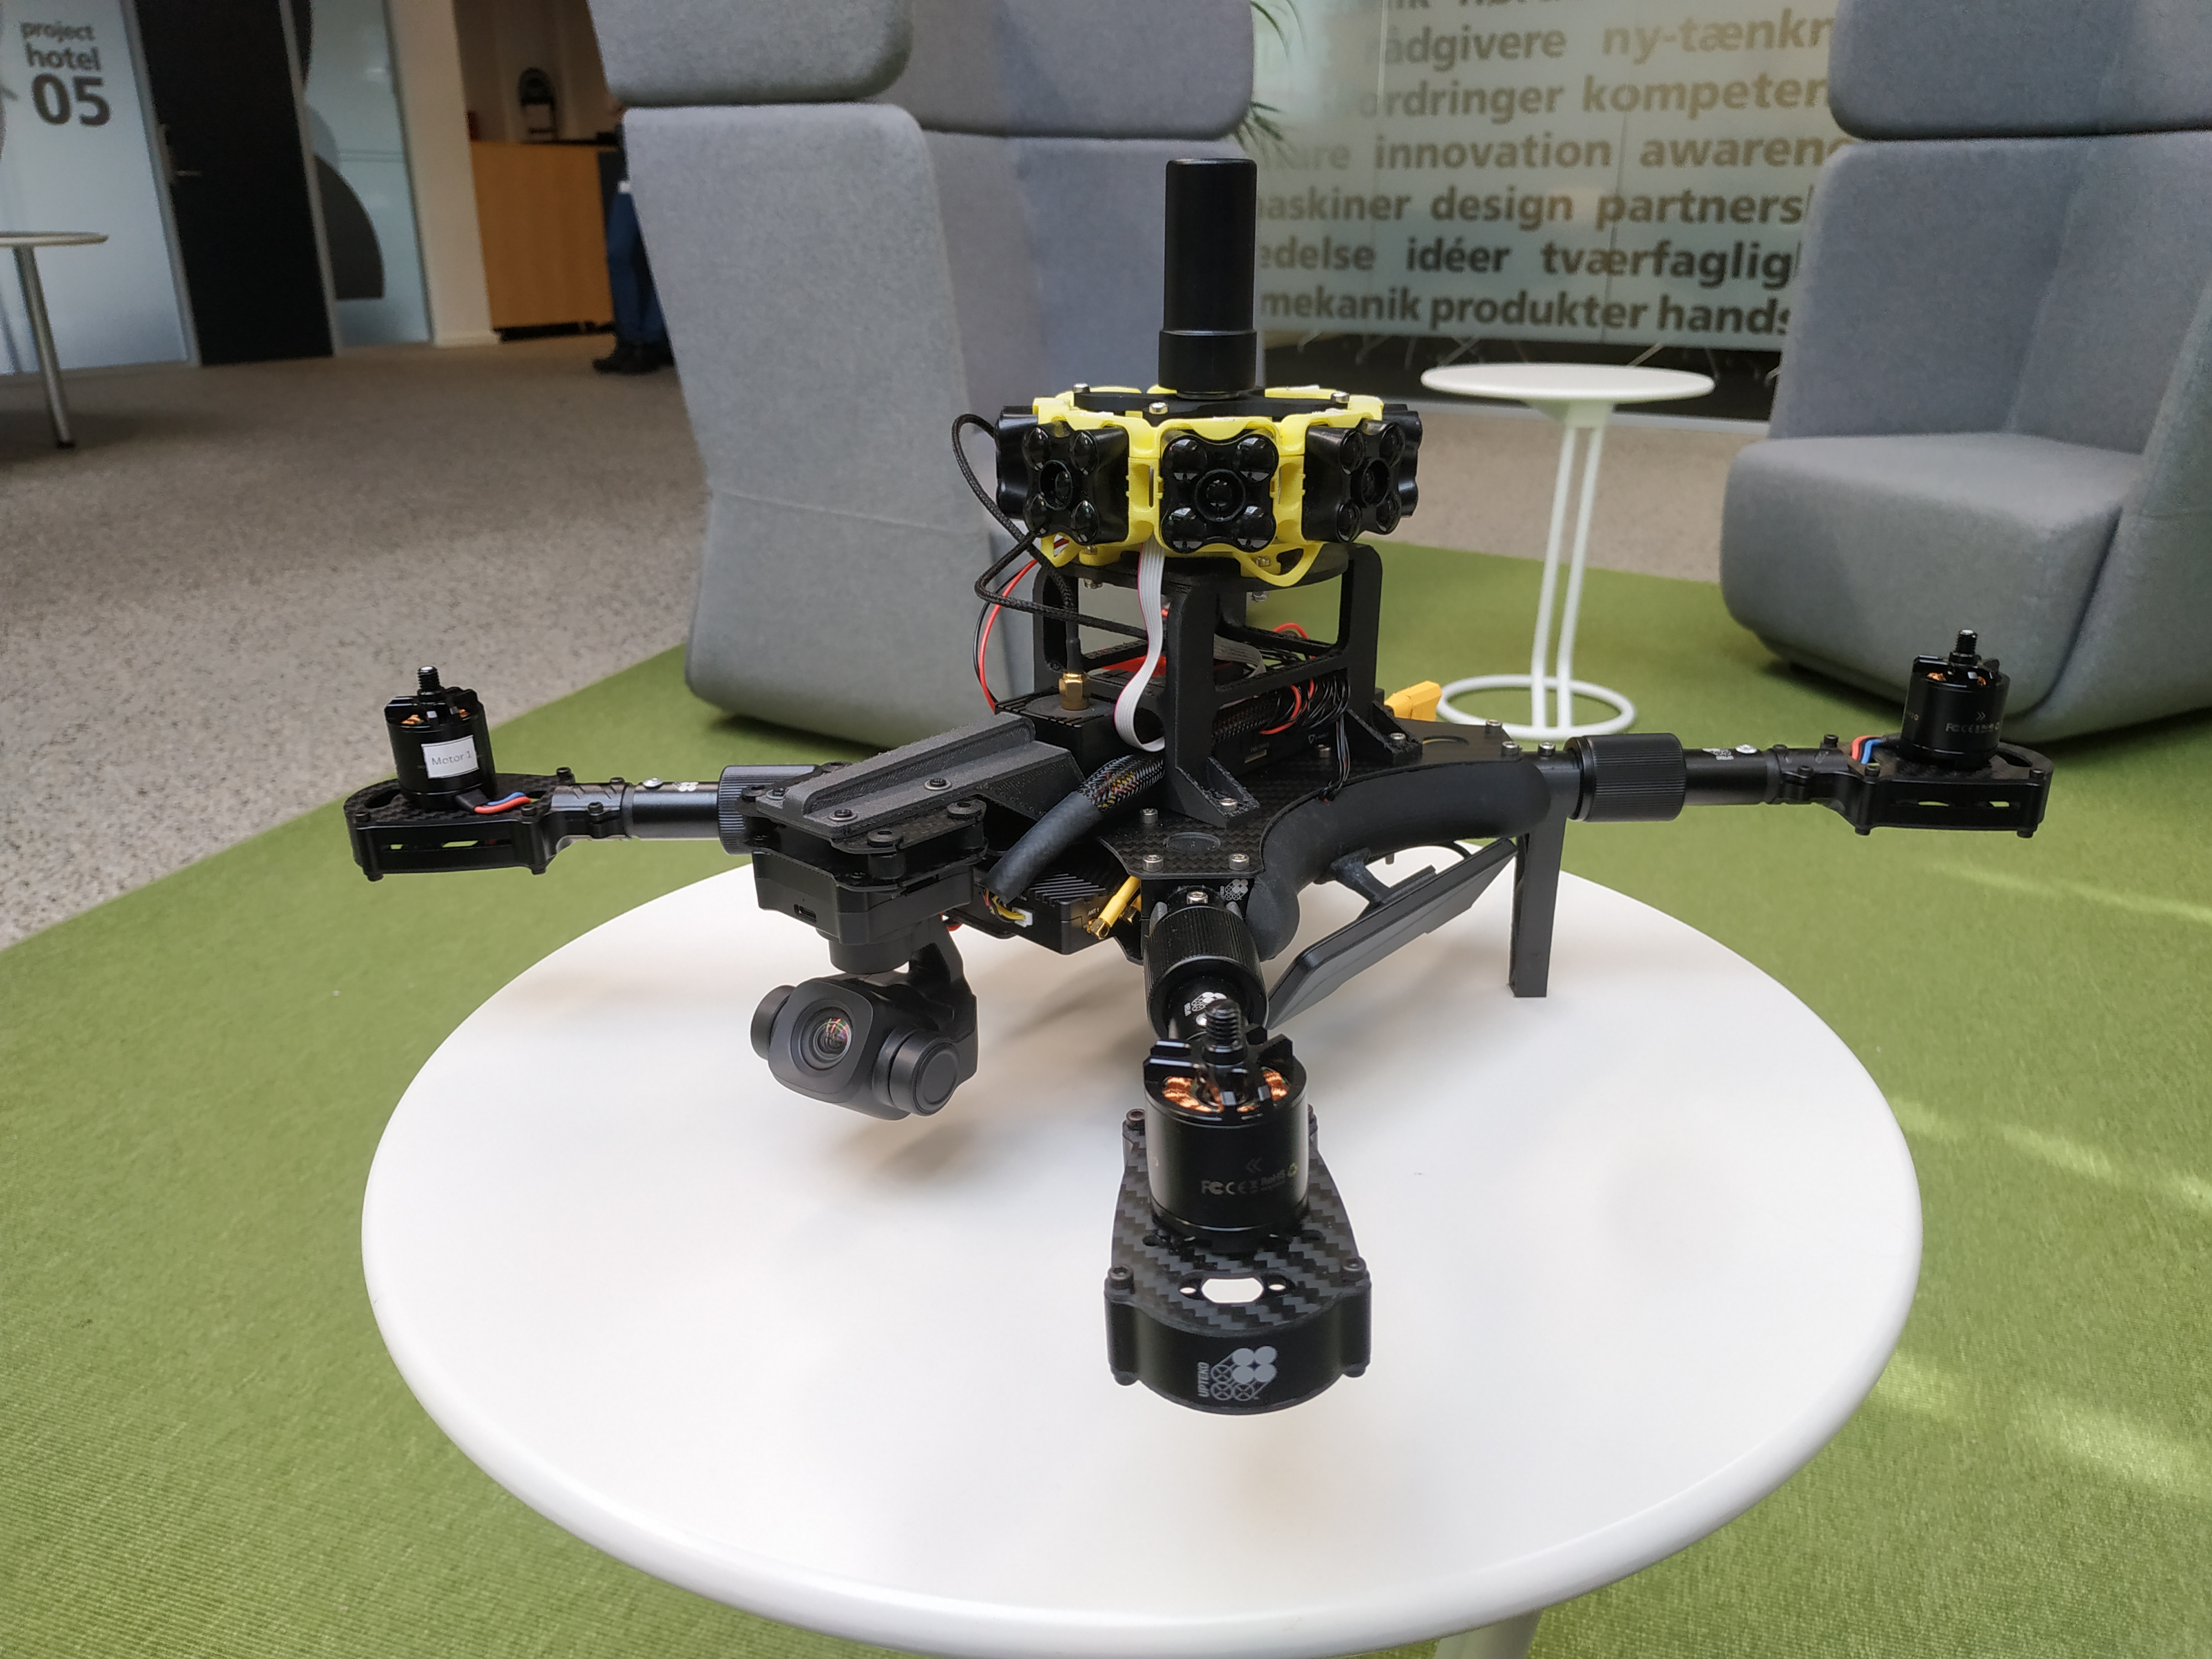
\includegraphics[width=\textwidth]{./projects/logviewer/drone_fl_view.jpg}
        \caption{Front left view}
    \end{subfigure}
    \hfill
    \begin{subfigure}[b]{0.475\textwidth}  
        \centering 
        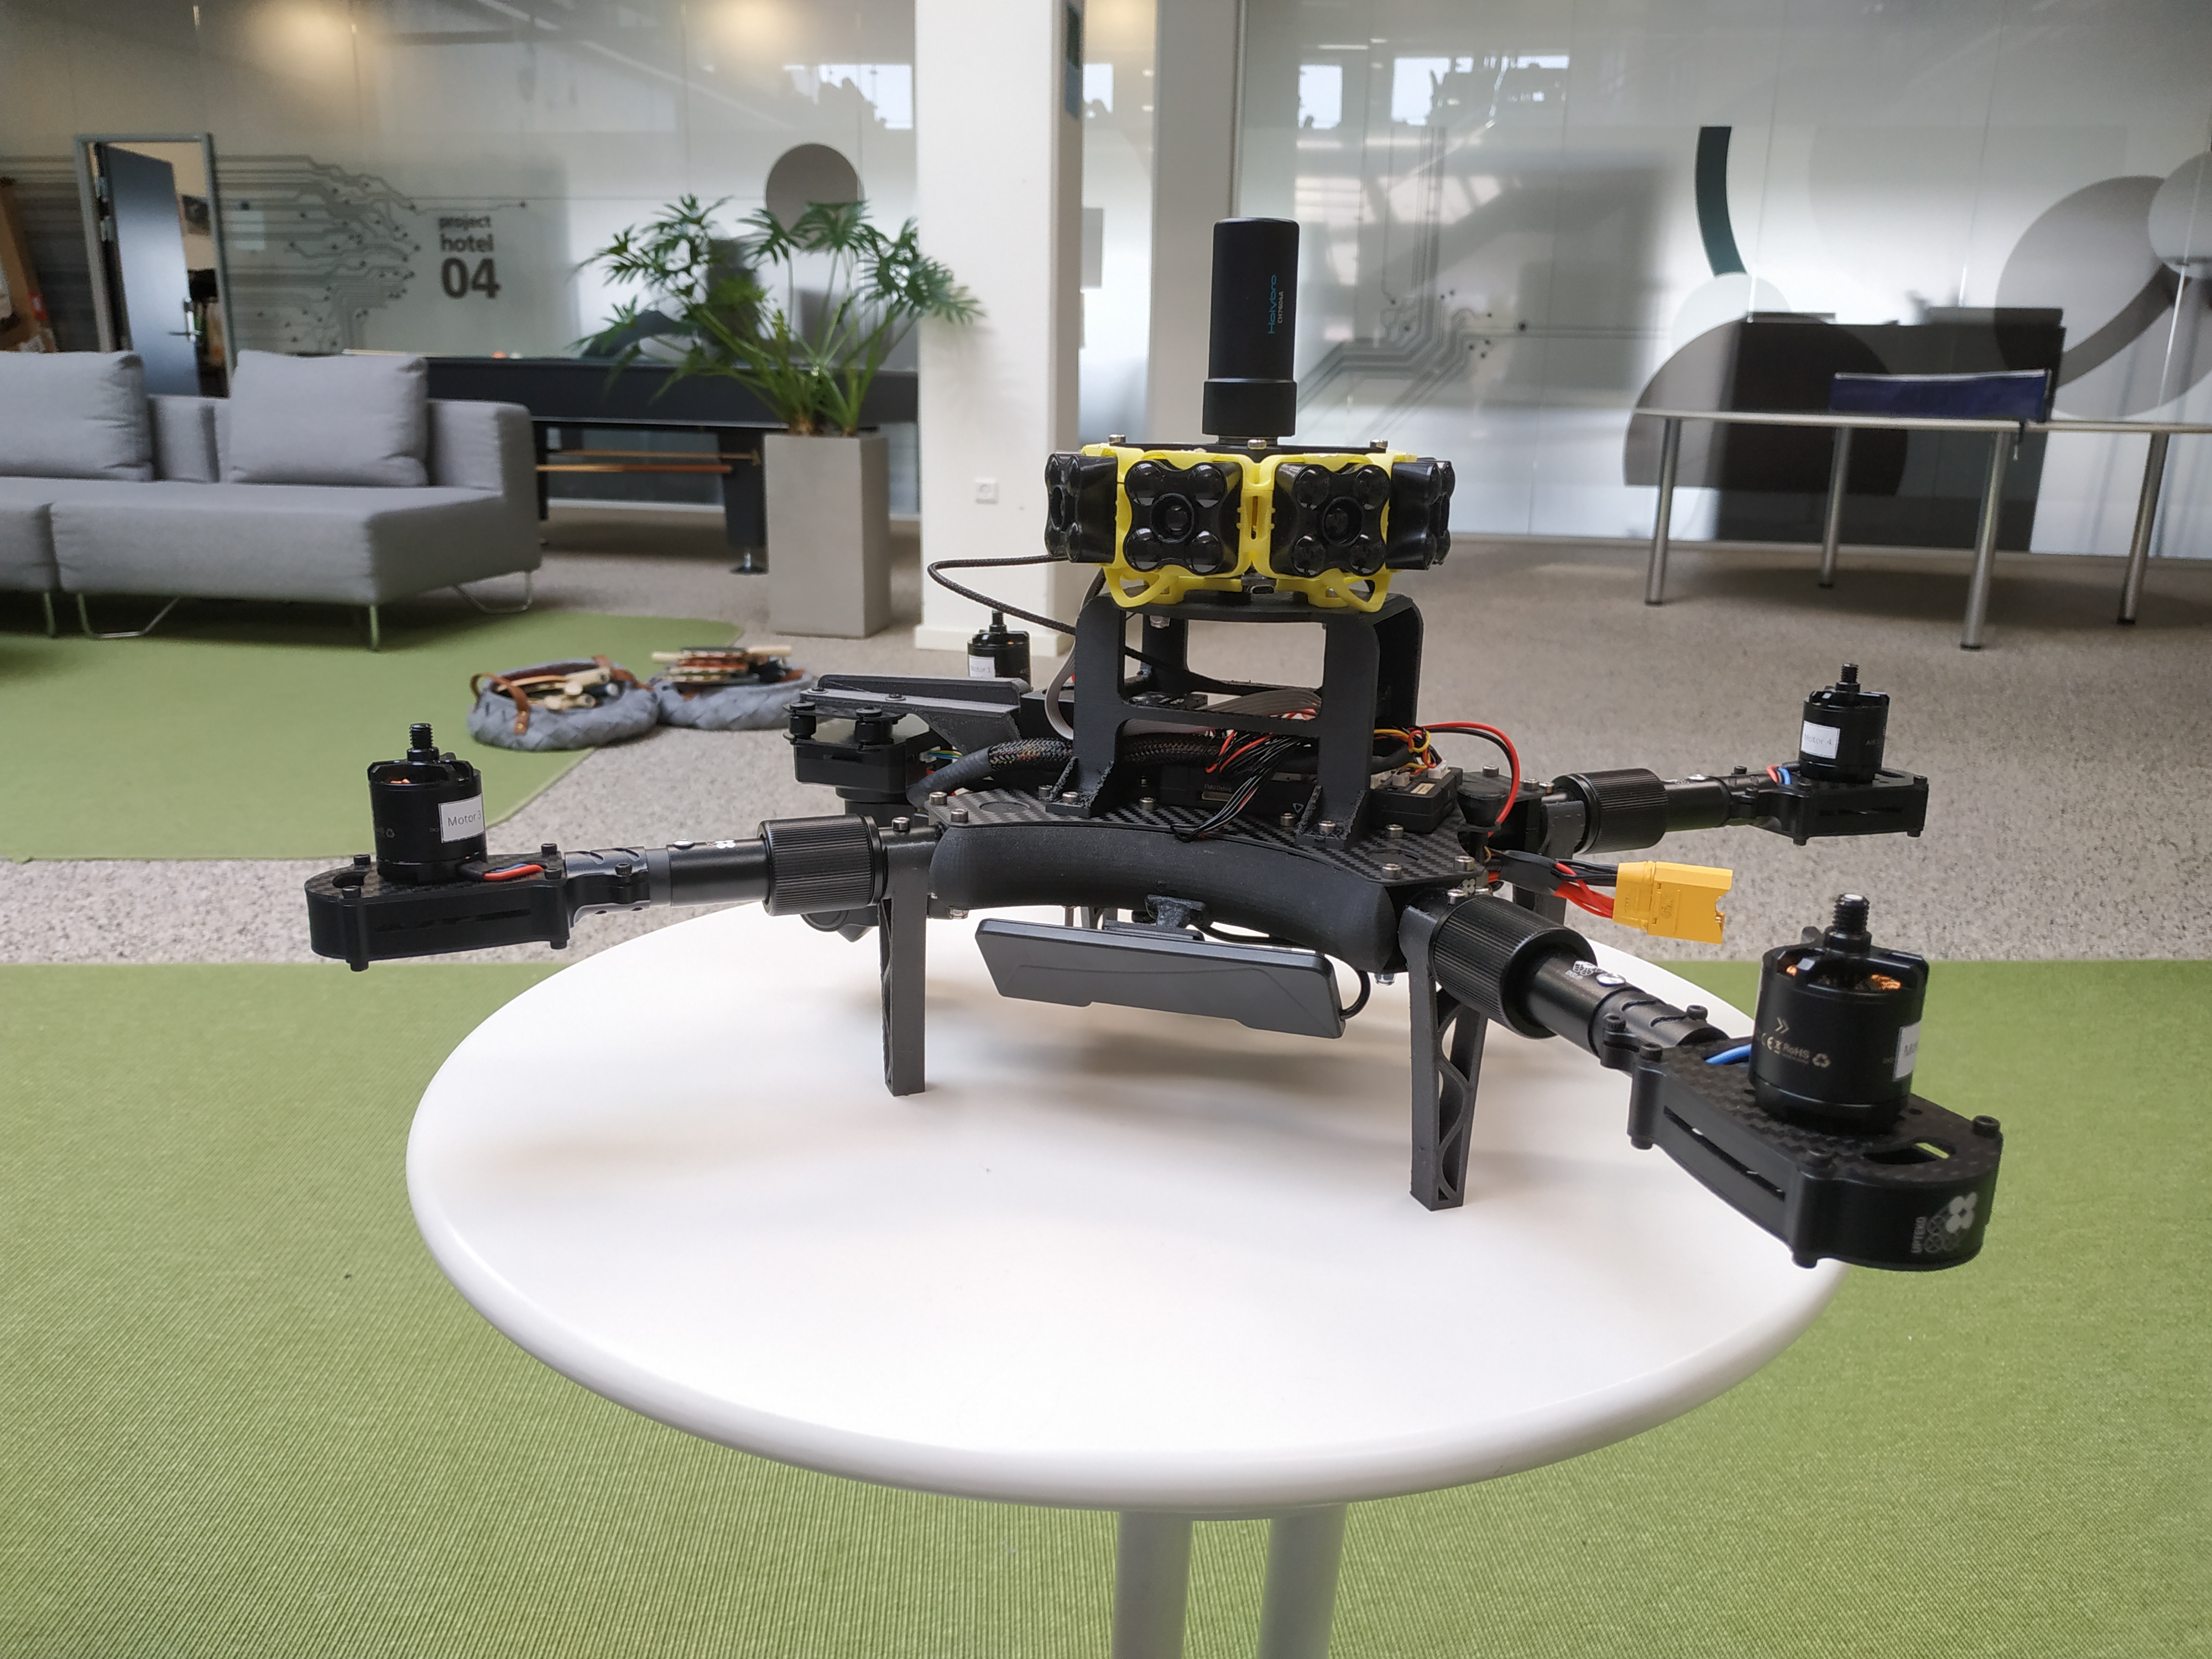
\includegraphics[width=\textwidth]{./projects/logviewer/drone_l_view.jpg}
        \caption{Left view}
    \end{subfigure}
    \vskip\baselineskip
    \begin{subfigure}[b]{0.475\textwidth}   
        \centering 
        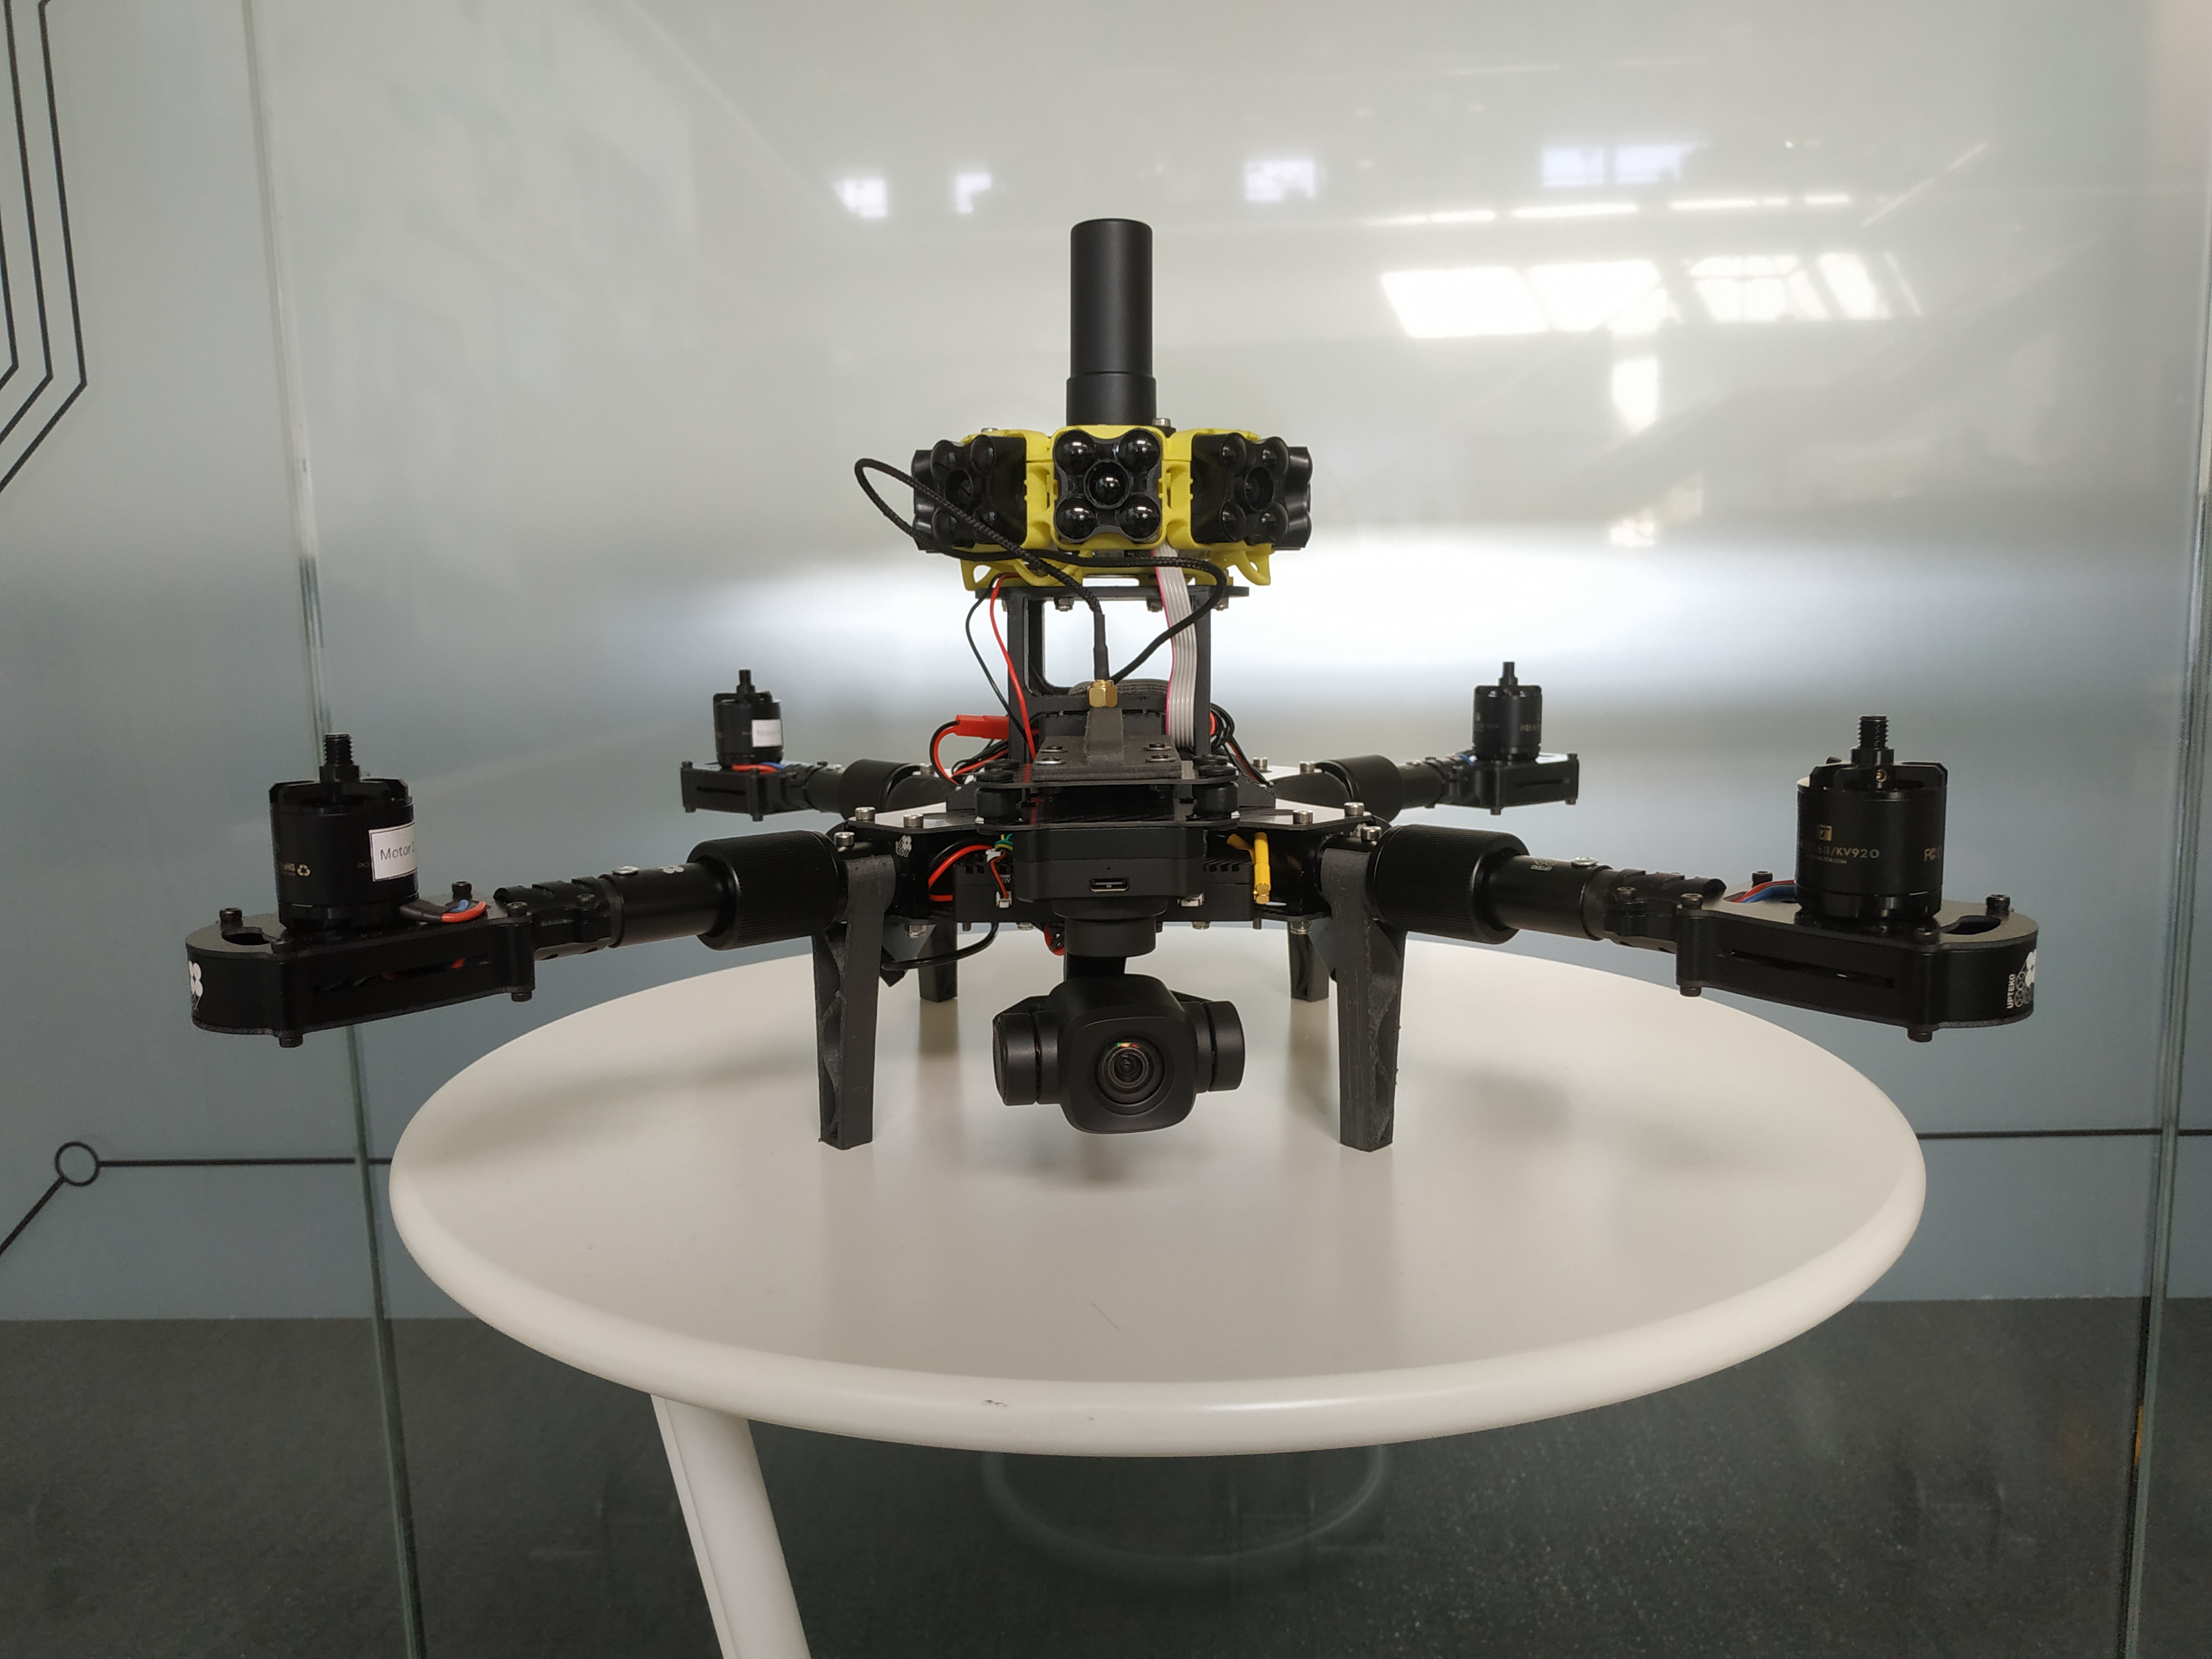
\includegraphics[width=\textwidth]{./projects/logviewer/drone_f_view.jpg}
        \caption{Front view}
    \end{subfigure}
    \hfill
    \begin{subfigure}[b]{0.475\textwidth}   
        \centering 
        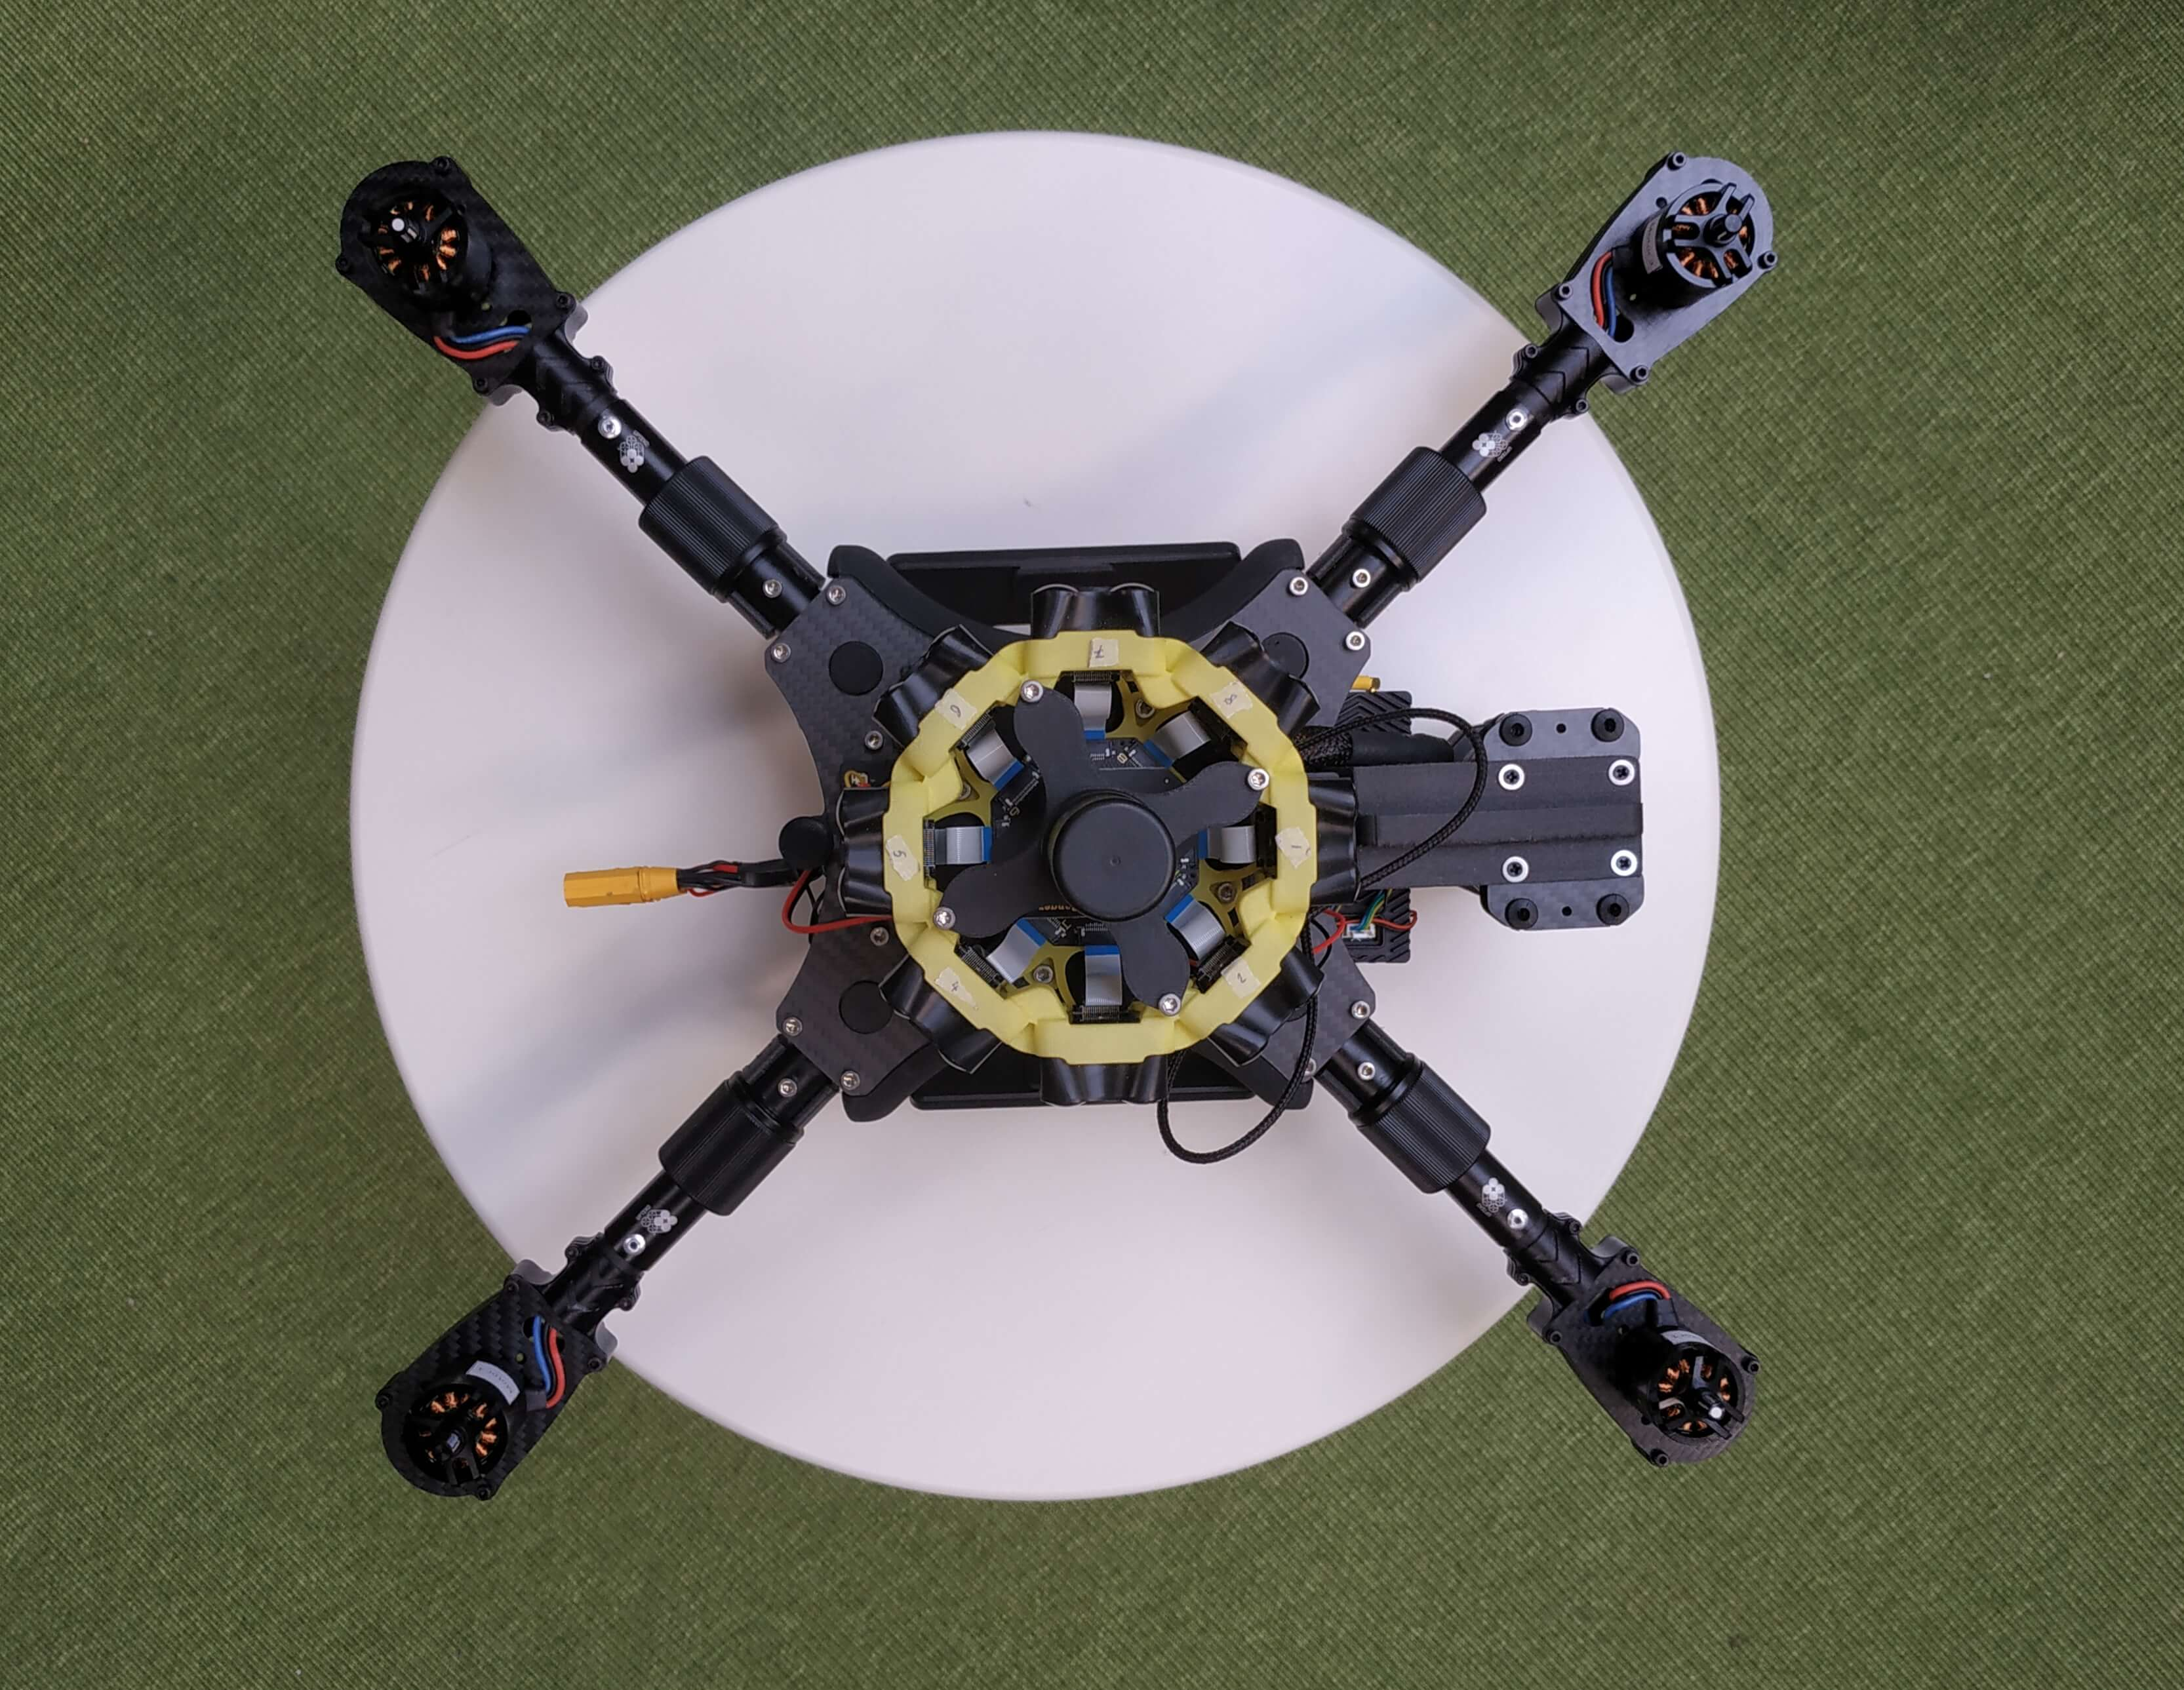
\includegraphics[width=\textwidth]{./projects/logviewer/drone_t_view.jpg}
        \caption{Top view}
    \end{subfigure}
    \caption{Larke Mini drone pictures with 360° degrees LIDAR mounted} 
\end{figure}


The drone successfully achieved its intended mission objectives. Whether it was aerial mapping and surveying, the drone effectively captured distance data.
My colleague Sebastian Duus ensured that the drone was in the optimal position for data acquisition, adjusting altitude and camera settings accordingly.

\subsection{Python Plotly Visualizer}
A graphical user interface is provided, leveraging \texttt{Plotly}\cite{plotly} library. The Logviewer import the \texttt{.csv} file as data.
Here is the \texttt{logfile.csv} header :
\begin{table}[H]
    \centering
    \begin{tabular}{|l|l|l|l|l|l|}
    \hline
    timestamp(ms) & PRX.D0 & PRX.D45 & PRX.D90 & PRX.D135 & PRX.D180 \\
    \hline
    PRX.D225 & PRX.D270 & PRX.D315 & ATT.Roll & ATT.Pitch & ATT.Yaw \\
    \hline
    \end{tabular}
    \caption{Plotly logviewer file header}
    \label{table:logfile_header}
\end{table}

The application is pretty simple : it use the timestamp as main variable to create animated data.
I created 3 main plots in th same window :
\begin{itemize}
    \item the distance sensors plot
    \item the roll and pitch attitude
    \item the yaw plot
\end{itemize}


The most valuable part of this application is the time slider that can be used to go back in time, pause and restart the view.
This way the data analysis is easy-to-use

\subsubsection{Final result}
% \begin{figure}[H]
%     \centering
%     \includegraphics{./projects/pmodnav/pmodnav_gui_record.gif}
%     \caption{Python GUI window GIF}
% \end{figure}

\section{Collision avoidance SITL}
\subsection{Environement description}
\subsubsection{Robot Operating System}
% ROS2 %
\texttt{ROS2} is an open-source framework for building robotic systems. It supports distributed systems, allowing communication between different components and nodes running on separate devices.
It provides a communication infrastructure for exchanging messages and supports various protocols. ROS 2 introduces a quality of service system for controlling communication behavior.
It includes real-time capabilities for time-critical applications. It supports multiple programming languages and emphasizes modularity and extensibility. ROS 2 comes with development tools and has an active community and ecosystem.
Overall, ROS 2 provides a powerful and versatile platform for developing robotic systems. Its distributed architecture, flexible communication infrastructure, real-time capabilities, language support, and extensibility make it a valuable tool for building complex and advanced robots.
\subsubsection{Gazebo}
% gazebo %
\texttt{Gazebo} is an open-source 3D simulation environment for robotics. It allows developers to create virtual worlds where they can simulate and test robots. Gazebo provides realistic physics-based simulations, visualizes the environment in 3D, and simulates sensors like cameras and lidars.
Users can model robots and their surroundings, integrate with the Robot Operating System (ROS), and extend its functionality using plugins. Gazebo has a supportive community and offers a wide range of resources for developers.
In summary, Gazebo is a valuable tool for simulating and evaluating robotic systems before deploying them in real-world environments.
\subsubsection{Ardupilot}
% ardupilot %
\texttt{Ardupilot} is open-source software used for controlling autonomous vehicles like drones. It includes firmware that runs on the vehicle's autopilot hardware, as well as ground control station software for mission planning and monitoring.
Ardupilot supports different flight modes, navigation based on waypoints, and telemetry for communication with the vehicle. It is compatible with various hardware platforms and can be customized and extended.
Ardupilot is widely used in drones and other vehicles, and it has a supportive community and extensive documentation. In summary, Ardupilot is a versatile and customizable software suite for autonomous vehicle control.

\subsection{Built-In Ardupilot collision avoidance}
The collision avoidance feature in Ardupilot is designed to enhance the safety and reliability of these vehicles by detecting and avoiding potential collisions with obstacles or other aircraft.

The collision avoidance system in Ardupilot relies on various sensors and algorithms to perceive the environment and make informed decisions about navigation. Some of the key components and techniques used in the Built-In Ardupilot collision avoidance include:

\begin{itemize}
    \item \underline{Sensor Inputs:} Ardupilot can interface with different types of sensors, including proximity sensors, lidar, sonar, and cameras. These sensors provide information about the surrounding environment and help in detecting obstacles.
    \item \underline{Obstacle Detection:} The collision avoidance system processes the sensor data to identify potential obstacles in the flight path. This can include buildings, trees, other aircraft, or any other objects that may pose a risk of collision.
    \item \underline{Path Planning:} Based on the environment map and the current position of the vehicle, Ardupilot generates a safe and collision-free path for the aircraft to follow. It considers factors such as obstacle proximity, vehicle speed, and maneuverability to calculate an optimal trajectory.
    \item \underline{Collision Avoidance Algorithms:} Ardupilot employs sophisticated algorithms to predict the future movement of obstacles and determine the best course of action to avoid collisions. These algorithms take into account the dynamics of the vehicle and the obstacles, allowing the autopilot to adjust the flight path accordingly.
\end{itemize}

% https://www.youtube.com/watch?v=W2ncr0DKWHE&ab_channel=IntelligentQuads

\begin{figure}[H]
    \centering
    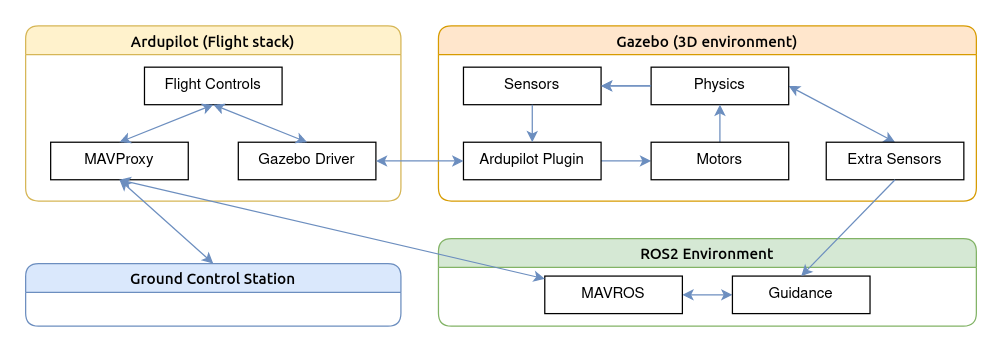
\includegraphics[width=0.65\linewidth]{./projects/ardupilot/sitl_overall.png}
    \caption{Software-In-The-Loop overall schematics}
\end{figure}

\subsection{Collision Avoidance ROS2 Migration}
